% chktex-file 44 32 36 38 18 11 8 26

\pagestyle{DS_FP}
%\NomPrenomNote{}

\bigskip

\section*{PARTIE A~--~Fiabilité des capteurs (Probabilités)}

\medskip

\emph{Dans cette partie, vous arrondirez toutes les valeurs à $10^{-4}$ si nécessaire.}

\medskip

 \begin{minipage}{0.48\textwidth}
Une entreprise installe des capteurs de température. Elle se fournit chez deux fabricants:
\begin{itemize}
    \item Fabriquant X: fournit 70\% des capteurs, avec un taux de défaillance de 2\%.    
    \item Fabricant Y: fournit 30\% des capteurs, avec un taux de défaillance de 5\%.
\end{itemize}

On note $D$ l'événement « le capteur est défectueux », $X$ l'événement « le capteur provient du fabriquant X » et $Y$ l'événement « le capteur provient du fabriquant Y ».

Un capteur est prélevé au hasard en sortie de chaîne.

\medskip

\begin{enumerate}[series=monDS, resume]
    \item Compléter l'arbre de probabilité ci-contre.
\end{enumerate}

\end{minipage}\hfill{}
\begin{minipage}{0.48\textwidth}
    \begin{blocvisiblex}[height=6]
    {\begin{center}
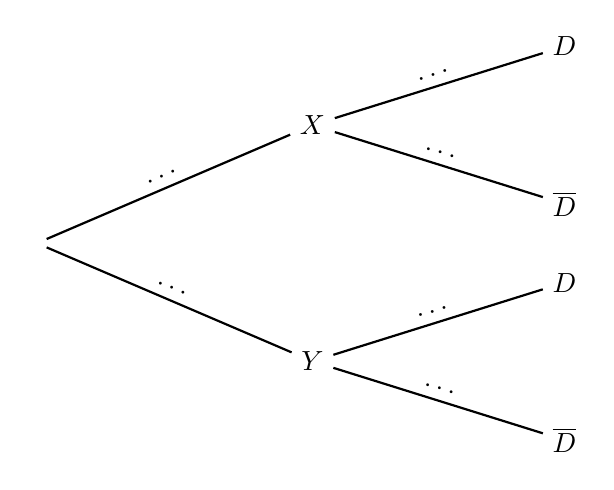
\begin{tikzpicture}[
    grow=right,     % On définit la croissance vers la droite
    % Réglages des distances entre les niveaux et les branches
    level 1/.style={sibling distance=3cm, level distance=3.5cm},
    level 2/.style={sibling distance=2cm, level distance=3.2cm},
    every node/.style={sloped}, % Aligne le texte sur les branches
    edge from parent/.style={draw, thick} % Ajoute une flèche au bout
]
% Racine
\node {} 
    child { node {$Y$}
        child { node {$\overline{D}$} 
            edge from parent node[above] {$\ldots{}$} }
        child { node {$D$} 
            edge from parent node[above] {$\ldots{}$} }
        edge from parent node[above] {$\ldots{}$} }
    child { node {$X$}
        child { node {$\overline{D}$} 
            edge from parent node[above] {$\ldots{}$} }
        child { node {$D$} 
            edge from parent node[above] {$\ldots{}$} }
        edge from parent node[above] {$\ldots{}$} }
    ;
\end{tikzpicture}
\end{center}}
\begin{center}
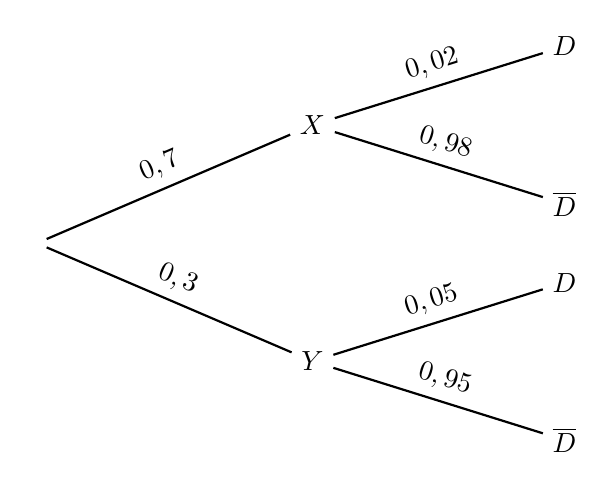
\begin{tikzpicture}[
    grow=right,     % On définit la croissance vers la droite
    % Réglages des distances entre les niveaux et les branches
    level 1/.style={sibling distance=3cm, level distance=3.5cm},
    level 2/.style={sibling distance=2cm, level distance=3.2cm},
    every node/.style={sloped}, % Aligne le texte sur les branches
    edge from parent/.style={draw, thick} % Ajoute une flèche au bout
    %edge from parent/.style={draw, -latex, thick} % Ajoute une flèche au bout
]
% Racine
\node {} 
    child { node {$Y$}
        child { node {$\overline{D}$} 
            edge from parent node[above] {$0,95$} }
        child { node {$D$} 
            edge from parent node[above] {$0,05$} }
        edge from parent node[above] {$0,3$} }
    child { node {$X$}
        child { node {$\overline{D}$} 
            edge from parent node[above] {$0,98$} }
        child { node {$D$} 
            edge from parent node[above] {$0,02$} }
        edge from parent node[above] {$0,7$} }
    ;
\end{tikzpicture}
\end{center}
    \end{blocvisiblex}
\end{minipage}



    
\begin{enumerate}[resume=monDS]
    \item Calculer la probabilité que le capteur soit défectueux et provienne du fabricant X.
     \begin{blocvisiblex}[height=2.5]
    {\quad}
    $P(X\cap D)=P(X) \times P_D(X)=0,7 \times 0,02=0,014$

    \smallskip
    La probabilité que le capteur soit défectueux et provienne du fabricant X est de $0,014$.
     \end{blocvisiblex}
     \medskip
    \item Calculer la probabilité que le module prélevé soit défectueux. Montrer que cette probabilité est égale à $0,029$.
    \begin{blocvisiblex}[height=2.5]
    {\quad}
    $P(D)=P(X\cap D)+P(Y\cap D)=P(X) \times P_D(X)+P(Y) \times P_D(Y)=0,7 \times 0,02+0,3 \times 0,05=0,029$

        \smallskip
    La probabilité que le capteur soit défectueux est de $0,029$.
    \end{blocvisiblex}
    \medskip
    \item Sachant que le capteur est défectueux, calculer la probabilité qu'il provienne du fabricant X.
    \begin{blocvisiblex}[height=2.5]
    {\quad}
    $P_X(D)=\dfrac{P(X\cap D)}{P(D)}=\dfrac{P(X) \times P_D(X)}{P(D)}=\dfrac{0,7 \times 0,02}{0,029}\approx 0,4828$

        \smallskip
    La probabilité que le capteur provienne du fabricant X sachant qu'il est défectueux est d'environ $0,4828$.
     \end{blocvisiblex}
     \medskip
    \item On installe un lot de 50 capteurs de manière indépendante. Soit X la variable aléatoire comptant le nombre de capteurs défectueux. Quelles sont les paramètres de la loi binomiale suivie par X ?
    \begin{blocvisiblex}[height=1]
    {\quad}
        Les paramètres de la loi binomiale suivie par X sont $n=50$ et $p=0,029$.
    \end{blocvisiblex}
    \medskip
    \begin{minipage}{0.46\linewidth}
             \item Déterminer la probabilité d'avoir au moins 3 capteurs défectueux dans ce lot.
             \medskip
    \end{minipage}\hfill{}
    \begin{minipage}{0.46\linewidth}
    \begin{blocvisiblex}[height=1]
    {\quad}
    $P(X\geq 3)=0,1767$
    \end{blocvisiblex}
    \medskip
    \end{minipage}
\bigskip
    \begin{minipage}{0.66\linewidth}
    \item On souhaite savoir à partir de combien de capteurs piochés, la probabilité d'avoir au moins 1 capteurs défectueux soit supérieure à 10\%. Déterminer à l'aide de Géogébra à partir de quelle valeur de $n$ la condition est satisfaite.
    \end{minipage}\hfill{}
    \begin{minipage}{0.26\linewidth}
    \begin{blocvisiblex}[height=1]
    {\quad}
    $n=4$
    \end{blocvisiblex}
    \end{minipage}

        \appelprof{}

     \end{enumerate}

\bigskip

\section*{PARTIE B~--~Étude d'un signal de commande (Analyse)}

La tension de commande d'un servomoteur est modélisée par la fonction g définie sur $\fo{0}{+\infty}$ par:

\[g(t)=(at+b)\cdot \e^{-0,2t}\qquad \text{où $a$, $b$ sont des constantes réelles}\]

     $t$ est le temps en millisecondes (ms) et     g(t) est la tension en volts (V) à l'instant $t$.

\subsection*{Etude d'un cas particulier}

    Dans cette partie uniquement, on donne $a=0$ et $b=12$. Ainsi la fonction $g$ s'exprime par: \fbox{$g(t)=12\cdot \e^{-0,2t}$}.

    
\begin{enumerate}[series=monDS, resume]
    \item Déterminer par le calcul une expression de la fonction dérivée $g'$ et montrer que $g'(t)=-2,4\cdot \e^{-0,2t}$.
    \begin{blocvisiblex}[height=2.5]
    {\quad}
    $g(t)= 12 \cdot \e^{-0,2t}$

    $g'(t)= 12 \cdot \Big(-0,2\cdot \e^{-0,2t}\Big)=-2,4\cdot \e^{-0,2t}$.
    \end{blocvisiblex}
    \medskip
    \item En déduire les variations de $g$ sur $\fo{0}{+\infty}$.
    \begin{blocvisiblex}[height=2.5]
    {\quad}
    $g'(t)$ est strictement négatif sur $\fo{0}{+\infty}$, ainsi $g$ est strictement décroissante sur $\fo{0}{+\infty}$.
    \end{blocvisiblex}

\end{enumerate}


\subsection*{Modélisation}

Dans cette partie, on considère que $a$ et $b$ sont des constantes réelles strictement positives, mais on ne connaît pas leurs valeurs.

Des études expérimentales ont permis de déterminer que:
\begin{itemize}
    \item la tension initiale $g(0)$ est de $2$ volts;
    \item la tension atteint un maximum au bout de $4$ ms.
\end{itemize}

La fonction $g$ est donc définie pour tout $t\geq 0$ par \fbox{$g(t)=(at+b)\cdot \e^{-0,2t}$}

\bigskip

\begin{enumerate}[series=monDS, resume]
    \begin{minipage}{0.48\textwidth}
    \item A l'aide des deux conditions expérimentales et à l'aide de Géogébra, déterminer les valeurs de $a$ et $b$.
\end{minipage}\hfill{}
\begin{minipage}{0.45\textwidth}
    \begin{blocvisiblex}[height=1.2]
    {$a=\dotfill \hspace{2cm} b=\dotfill$}
    $a=2 \hspace{2cm} b=2$
    \end{blocvisiblex}
\end{minipage}
    \appelprof{}
\end{enumerate}

\bigskip

Dans la suite de l'exercice on considèrera la fonction $g$ définie sur $\fo{0}{+\infty}$ par $g(t)=2(t+1)\cdot \e^{-0,2t}$.


\medskip


\begin{enumerate}[series=monDS, resume]
     
    \begin{minipage}{0.75\linewidth}
           \item Déterminer grâce à Géogébra à partir de quelle valeur de $t$ la tension $g(t)$ devient inférieure à 0,5 volt. (On donnera une valeur approchée à $10^{-2}$ près.)

    \end{minipage}\hfill{}
    \begin{minipage}{0.21\linewidth}
    \begin{blocvisiblex}[height=1]
    {\quad}
    $t\approx 22,77$ ms.
    \end{blocvisiblex}
\end{minipage}

    \item Calculer l'énergie totale dissipée $E=\int_0^{10} g(t) \, \dt$ entre $t=0$ et $t=10$ sachant qu'une primitive de $g$ est donnée par $G(t)=-10(t+6)\cdot \e^{-0,2t}$.
    \begin{blocvisiblex}[height=1.2]
    {\quad}
    L'énergie totale dissipée entre $t=0$ et $t=10$ est $E=G(10)-G(0)=\dotfill 38,35$ joutes.
    \end{blocvisiblex}
\end{enumerate}
    

\pagebreak

\thispagestyle{DS_LP}

%\thispagestyle{DS_LP}
\section*{PARTIE C~--~Débit d'une liaison satellite (Suites)}

Lors d'un orage, le débit d'une antenne chute progressivement. Initialement, le débit est de 100 Mbit/s. À chaque seconde, le signal perd 15\% de sa puissance.

Soit $v_n$ le débit après $n$ secondes.


\begin{enumerate}[series=monDS, resume]
    \item Justifier que la suite $(v_n)$ vérifie la relation de récurrence $v_{n+1}=0,85\cdot v_n$.
    \begin{blocvisiblex}[height=3.5]
    {\quad}
    La suite $(v_n)$ vérifie la relation de récurrence $v_{n+1}=0,85\cdot v_n$ car à chaque seconde, le signal perd 15\% de sa puissance.

    On a donc $v_{n+1}=v_n-0,15\cdot v_n=0,85\cdot v_n$.

    \end{blocvisiblex}
    \medskip
    \item Déterminer la nature de la suite $(v_n)$. 
    \begin{blocvisiblex}[height=2]
    {\quad}

    La suite $(v_n)$ est de la forme $v_{n+1}=q \times v_n$ avec $q=0,85$ constant, donc c'est une suite géométrique de raison $0,85$ et de premier terme $v_0=100$.
    \end{blocvisiblex}
    \medskip
    \item Exprimer $v_n$ en fonction de $n$. 
    \begin{blocvisiblex}[height=2]
    {\quad}
    $(v_n)$ est une suite géométrique de raison $0,85$ et de premier terme $v_0=100$, donc pour tout $n$ entier naturel, on a $v_n=v_0 \times q^n=100 \times 0,85^n$.
    \end{blocvisiblex}
    \medskip
    \begin{minipage}{0.45\textwidth}
    \item Compléter l'algorithme ci-dessous qui calcule le nombre de cycles d'horloges nécessaires pour que la quantité de données dans le buffer soit inférieure à 10 Mbit/s.

    \end{minipage}\hfill{}
    \begin{minipage}{0.46\textwidth}
    \begin{tcblisting}{%
  listing only,
  colback=white, 
  colupper=black, 
  title=Algorithme de recherche de seuil,
  boxsep=0pt,
  left=5mm,
  listing options={
    numbers=none,
    basicstyle=\ttfamily,
    escapeinside={(*}{*)},
    literate={<-}{{$\bm{\leftarrow}$}}2, % Ajout d'un petit espace après la flèche
    frame=none % Supprime le cadre interne de listings
    }
}
n <- 0
v <- 100
tant que (*\trou{v >= 10}*):
        v <- (*\trou{0,85 * v}*)
        n <- (*\trou{n + 1}*)
print(n)
\end{tcblisting}
    \end{minipage}
    \medskip

    \end{enumerate}

\bigskip



